\chapter{L'équation de la lentille}
% Plan pour cette section: Dériver eq de la lentille et alpha
% Intro général: deflection de la lumière
%% Approcha a l'intro -> contexte historique à notre pensée sur la déviation de la lumière
%%% Réfraction 
%%%% Ptolémé (Optic, Grèce Antique)
%%%% Ibn Sahl (c. 940 - 1000)
%%%% Snell (1621)-Descartes(1637)
%%%% Principe de Fermat pour expliquer ce phénomène (lettre en 1657, mémoire en 1662)
%%%% Euler (1744) - Lagrange (1760) -> Principe de moindre action et sa solution
%%%% Équations de Maxwell (1861)

%%% déviation de la lumière par la gravité
%%%% Soldner, J. G. v. (1801–1804). "On the deflection of a light ray from its rectilinear motion, by the attraction of a celestial body at which it nearly passes by". Berliner Astronomisches Jahrbuch: 161–172.
%%%% Einstein 1911
%%%% Einstein 1915 (GR)
%%%% Eddington takes photograph of eclipse 1919
%%%% 1936 letter from Einstein at the request of 
%%%% Fritz Zwicky is first to postulate grav lensing idea in 1937i Zwicky, F. (1937) Nebulae as gravitational lenses. Physical Review, 51 (4). p. 290. ISSN 0031-899X
%%%% 1964 Refsdal (H0 and possibility to measure mass)
%%%%%% (Shapiro time delay (1964))
%%%% Fisrt gravitational lens discovered 1979 (double imaged quasar) https://www.nature.com/articles/279381a0
%%%% Then explosions of studies durings the 2000s on how to model things.

%%% Dark matter 
%%%% Zwicky 1933
%%%% Lambda CDM?
%%%% 

% Copied from https://royalsocietypublishing.org/doi/10.1098/rsta.2009.0209
%Henry Cavendish in 1784 is credited with the first (unpublished) calculation of the deflection angle 
%δ of a corpuscular light ray following a hyperbolic trajectory and the origin of the 
%(Newtonian) equation δ=2GM/Rc2. Subsequently, von Soldner (1804) published a similar calculation 
%deriving a deflection of 0.84 arcsec for stars viewed close to the limb of the Sun.

%Le principe de Fermat énonce que la trajectoire de la lumière, ou d'un 
%photon, doit suivre une trajectoire qui extrémise la durée de la trajectoire. 
%Ce principe mathématique, qui est un exemple du principe plus général de moindre action 
%développé par Lagrange en 1756, permet de décrire la trajectoire de la lumière 
%par l'entremise d'un simple indice $n$ (indice de réfraction) dans 
%lequel se cache toute la physique microscopique (ou macroscopique) 
%d'où émerge le phénomène qui nous intéresse. 


%L'expédition organisée par sir Arthur Eddington
%avait pour but d'observer 
%l'éclipse totale du 29 mai 1919 à partir de l'île de Prìncipe 
%dans le golfe de Guinée et de Sobral au nord du Brésil 
%\citep{Eddington1919}. Les photographes de l'éclipses prisent , bien qu'imprécises, 
%ont permis de valider la prédiction d'Einstein faite 
%en 1911 que la position observée d'une étoile serait déplacée de 
%$\delta \theta \approx 1.75'' \frac{R}{R_\odot}$ 
%durant une eclipse \citep{Dyson1920}, soit 2 fois plus 
%que ce qui est prédit par la théorie newtonienne.

%Dans l'intérêt de rendre ce manuscrit complet, je dérive à partir de principes 
%premier les deux équations centrales qui nous permettent 
%d'étudier les lentilles gravitationnelles.
Dans cette section, je dérive les équations centrales qui nous permettent 
d'étudier les lentilles gravitationnelles de type galaxie-galaxie.
Des traitements similaires 
peuvent être trouvé dans les manuels de références de \citet{Meneghetti2013} et 
\citet{Carroll2003}.


Supposons qu'un photon est sur une trajectoire parallèle à l'axe de 
visée $\mathbf{e}_{\parallel}$ d'un observateur sur Terre. 
Supposons de plus qu'un champ gravitationnel $\Phi$ a pour effet de courber la 
trajectoire de ce photon entre son point d'origine $A$ et son point d'arrivé $B$.
On définit l'angle de déviation comme la déviation totale de cette trajectoire 
dans la direction perpendiculaire à l'axe de visée de l'observateur. 
Selon nos suppositions, cette déviation s'écrit
\begin{equation}\label{eq:alpha}
        \boldsymbol{ \alpha} = - \int_{\lambda_A}^{\lambda_B} \ddot{\mathbf{x}} \times \mathbf{e}_{\parallel} d\lambda,
\end{equation}
où $\lambda$ paramétrise la trajectoire du photon, et $\mathbf{x}$ est la positon du photon. 
Le signe négatif nous indique qu'on prend la perspective de l'observateur. 

Pour résoudre l'intégrale \eqref{eq:alpha}, on doit déterminer la forme de 
la trajectoire des photons dans un champ gravitationnel caractérisé par un 
indice de réfraction $n$. 
Le principe de Fermat stipule que la lumière suit une trajectoire qui extrémise
la durée du parcours entre deux points. 
Dans le language du calcul 
des variations, la variation de la durée $T$ s'écrit
\begin{equation}\label{eq:Fermat}
        \delta T =  \delta \int_{A}^{B} n(\mathbf{x}(\ell)) \frac{d\ell}{c}= 0,
\end{equation}
où $\ell$ est un élément de longueur sur la trajectoire.
Pour déterminer l'indice de réfraction du champ gravitationnel d'une galaxie, 
on doit utiliser le formalisme de la relativité générale. Selon le principe 
d'équivalence (fort), 
l'effet d'un champ gravitationnel est localement 
indistinguable d'une accélération causée par la courbure 
de l'espace-temps décrit par 
une métrique $g_{\mu \nu}$. 
La trajectoire d'un photon se trouve alors en cherchant 
les géodésiques de cet espace-temps. 
On fait l'approximation 
que le potentiel $\Phi$ d'une galaxie est celui d'un gas parfait, c'est-à-dire 
qu'il satisfait une équation de Poisson
\begin{equation}\label{eq:Poisson}
       \grad^{2}\Phi = 4\pi G \rho .
\end{equation} 
Dans la limite où ce potentiel est faible $\displaystyle \frac{2\Phi}{c^{2}} \ll 1$, la 
métrique $g_{\mu \nu}$ est décrite par une expansion au premier ordre autour de la 
métrique de Minkowsky $\eta_{\mu\nu}$
\begin{equation}\label{eq:metrique}
        ds^2 = g_{\mu\nu}dx^{\mu}dx^{\nu} \approx \left( 1 + \frac{2\Phi}{c^{2}} \right)c^{2}dt^{2} - \left( 1 - \frac{2\Phi}{c^{2}} \right)d\mathbf{x}^{2}.
\end{equation} 
Ici, j'ai choisit arbitrairement la signature $(+,-,-,-)$ pour la métrique.
Puisqu'un photon suit une géodésique de l'espace-temps $ds^{2} = 0$, on peut déterminer 
$n$ en réarrengeant l'équation \eqref{eq:metrique}
\begin{equation}\label{eq:n}
        n = c \left( \frac{\lVert d \mathbf{x} \rVert}{dt}  \right)^{-1} \approx  1 - \frac{2\Phi}{c^{2}}.
\end{equation} 
En réécrivant l'élément de longueur $d\ell$ en terme du 
paramètre de la trajectoire $\lambda$
\begin{equation}\label{eq:ell}
        d\ell = \left\lVert\frac{d  \mathbf{x} }{d\lambda} \right\rVert d\lambda,
\end{equation} 
on peut réécrire l'équation \eqref{eq:Fermat} sous la forme
\begin{equation}\label{eq:Fermat2}
        \delta \int_{\lambda_A}^{\lambda_B} n(\mathbf{x}) \lVert \mathbf{\dot{x}} \rVert d\lambda = 0.
\end{equation} 
Par correspondance avec la fonctionnelle de l'action 
$J(x) = \int_{\lambda_0}^{\lambda_1} \mathcal{L}(\lambda,\, x,\,\dot{x}) d\lambda$ 
on trouve que 
le lagrangien de la trajectoire s'écrit 
\begin{equation}\label{eq:lagrangien}
        \mathcal{L} = n(\mathbf{x})  \sqrt{\dot{x}^{2}}.
\end{equation} 
La trajectoire qui satisfait \eqref{eq:Fermat} 
est une solution des équations d'Euler-Lagrange
\begin{equation}\label{eq:EulerLagrange}
        \frac{d }{d \lambda} \frac{\partial \mathcal{L}}{\partial \dot{\mathbf{x}}} - \frac{\partial \mathcal{L}}{\partial \mathbf{x}} = 0.
\end{equation} 
On a donc
\begin{equation}\label{eq:EulerLagrange2}
        \frac{d }{d \lambda} n \frac{\dot{\mathbf{x}}}{\lVert \dot{\mathbf{x}} \rVert}- \lVert \dot{\mathbf{x}} \rVert \grad n = 0 ,
\end{equation} 
Puisque le choix du paramètres $\lambda$ est libre, on peut le choisir tel 
que $\lVert \dot{\mathbf{x}} \rVert = 1$ en tout point de la trajectoire. Ainsi,
\begin{equation}\label{eq:EulerLagrange3}
\begin{aligned}
        \frac{d }{d \lambda} n \dot{\mathbf{x}} -  \grad n &= 0 \\
        \implies n \ddot{\mathbf{x}} + (\grad n \cdot \dot{\mathbf{x}}) \dot{\mathbf{x}} - \grad n &= 0
\end{aligned}
\end{equation} 

À ce point de la dérivation, on utilise l'approximation de Born. 
C'est-à-dire qu'on approxime la trajectoire 
du photon comme une ligne droite sur l'axe de visée $\mathbf{e}_{\parallel}$. 
Cette approximation est justfiée 
dans le contexte des lentilles gravitationnelles de type galaxie-galaxie, 
puisque les angles de déviation sont généralement de 
l'ordre de l'arcseconde ou plus petit. 
Comme, le vecteur $\dot{\mathbf{x}}$ est tangent à la trajectoire du photon, 
on obtient
\begin{equation}\label{eq:sol}
        \ddot{\mathbf{x}} \times \mathbf{e}_{\parallel} = \frac{1}{n} \grad_\perp n = \grad_\perp \log n
        \approx -\frac{2}{c^{2}}\grad_{\perp} \Phi
\end{equation} 
On note que le facteur 2 qui apparaît dans l'équation \eqref{eq:sol} est un 
effet qui vient de la relativité générale. Ce facteur corrige la solution 
que l'on aurait obtenu avec une dérivation classique (newtonienne).


On est maintenant en mesure de calculer l'angle de déviation. 
J'introduit le paramètre d'impact $\boldsymbol{\xi}$ qui est la distance perpendiculaire entre 
la position d'origine du photon sur le plan de la lentille  
et l'axe de visé. Cette distance peut être interprétée à l'aide du schéma dans la 
Figure \ref{fig:cartoon}.
Dans le cas où le potentiel est généré par une masse $M$ ponctuelle, ç.-à-d. qu'on 
suppose $\rho = M\delta^{3}(\mathbf{x})$ où $\delta $ est la fonction delta de Dirac, 
alors le potentiel qui satisfait l'équation de Poisson est 
la fonction de Green 
$\displaystyle \Phi = -\frac{GM}{\sqrt{ \xi^{2} + z^{2}}}$, où $z$ est la coordonné 
sur l'axe de visée. L'équation \eqref{eq:alpha} se réécrit finalement
\begin{align}
\nonumber
        \boldsymbol{ \alpha}(\boldsymbol{ \xi} ) &= -\frac{2GM}{c^{2}} \int_{-\infty }^{\infty }  \frac{\partial}{\partial \boldsymbol{\xi} }\frac{1}{(\xi^{2} + z^{2})^{1/2}}dz \\
\nonumber
        &= \frac{2GM}{c^{2}} \boldsymbol{ \xi}  \int_{-\infty }^{\infty } \frac{1}{(\xi^{2} + z^{2})^{3/2}}dz  \\
\label{eq:deflection approx}
        \implies \boldsymbol{ \alpha}(\boldsymbol{ \xi})  &= \frac{4GM}{c^{2}  \xi^{2} } \boldsymbol{ \xi}
\end{align} 
Cette solution se généralise naturellement à un profil de masse quelconque en assumant 
qu'il s'exprime comme une somme d'élément de masses $dm = \Sigma d^{2}\boldsymbol{ \xi}'$ 
où $\Sigma = \int \rho dz$ est un densité surfacique de masse. 
L'angle de déviation total mesuré à un point $\boldsymbol{\xi} $ est alors une convolution 
sur tout le plan de la lentille (mince) puisque l'équation \eqref{eq:deflection approx} dépend 
linairement de la masse $M$:
\begin{equation}\label{eq:alpha physique}
        \boldsymbol{ \alpha} (\boldsymbol{ \xi} ) = \frac{4 G}{c^{2}} 
        \int_{\mathbb{R}^{2}} \Sigma (\boldsymbol{ \xi} ')
        \frac{\boldsymbol{ \xi}  - \boldsymbol{ \xi} '}{\lVert \boldsymbol{ \xi}  - \boldsymbol{ \xi} ' \rVert^{2}}d^{2}\boldsymbol{ \xi} '
\end{equation} 

Cette déviation nous permet alors de relier le plan de la lentille et le plan de la source. 
Pour ce faire, on doit retrouver la position angulaire 
d'un point lumineux à la source $\boldsymbol{\beta}$ à partir de sa position angulaire
observée $\boldsymbol{ \theta} $ et de nos connaissances sur la déviation $\boldsymbol{ \alpha}$. 
On assume que les distances $D_{\ell}$, $D_s$ et $D_{\ell s}$ sont beaucoup 
plus grandes que les distances perpendiculaires $\boldsymbol{ \xi} $ ou $\boldsymbol{ \eta} $ 
(voir figure \ref{fig:cartoon}). 
Pour les objets qui nous intéresses, les distances parallèles à l'axe de visée sont généralement 
de l'ordre du Gpc, alors que les distances perpendiculaire sont généralement 
de l'ordre du kpc, soit 6 ordres de grandeurs de différences.
Ainsi, on peut faire l'argument géométrique
\begin{align}
\nonumber
       D_{s} \boldsymbol{ \theta} &= \boldsymbol{ \eta}' \\   
\nonumber
       D_{s} \boldsymbol{ \beta} &= \boldsymbol{ \eta} \\   
\nonumber
       D_{\ell s} \boldsymbol{ \alpha} &= \boldsymbol{ \eta}' - \boldsymbol{ \eta}  \\   
\label{eq:lens equation}
       \implies D_s \boldsymbol{ \beta} &= D_s \boldsymbol{ \theta} - D_{\ell s} \boldsymbol{ \alpha}   
\end{align} 
C'est l'équation maîtresse qui nous permet de tracer les rayons lumineux d'une source 
vers un détecteur fictif dans nos simulations.

Lorsqu'on étudie des images, il est généralement plus utile de travailler directement à partir 
du système de coordonnées angulaires $\boldsymbol{ \theta}$ plutôt que des dimensions physiques 
$\boldsymbol{ \xi}$ qui requièrent une caractérisation précise de la distance entre 
l'observateur et la lentille $\boldsymbol{ \xi}  = D_\ell \boldsymbol{ \theta} $.
On peut absorber cette distances dans un préfacteur qui rend les expressions 
\eqref{eq:alpha physique} et \eqref{eq:lens equation} adimensionnelles.
On introduit la densité critique 
\begin{equation}\label{eq:densite critique}
        \Sigma_c = \frac{c^2}{4 \pi G}\frac{D_{s}}{D_{\ell s} D_\ell}
\end{equation} 
et la convergence $\displaystyle \kappa(\boldsymbol{ \theta} ) = \frac{\Sigma(\boldsymbol{ \theta})}{\Sigma_c}$, 
de sortes qu'on obtient l'angle réduit
\begin{equation}\label{eq:alpha adim}
        \hat{\boldsymbol{ \alpha}} (\boldsymbol{ \theta}) = \frac{1}{\pi}\int_{\mathbb{R}^{2}} \kappa(\boldsymbol{ \theta} )
        \frac{\boldsymbol{ \theta} - \boldsymbol{ \theta}'  }{\lVert \boldsymbol{ \theta} - \boldsymbol{ \theta}' \rVert  } d^{2}\boldsymbol{ \theta}'   
\end{equation} 
qui satisfait
\begin{equation}\label{eq:lens equation adim}
        \boldsymbol{ \beta} = \boldsymbol{ \theta} - \hat{\boldsymbol{ \alpha}}(\boldsymbol{ \theta})    
\end{equation}

\begin{figure}[H]
        \centering
        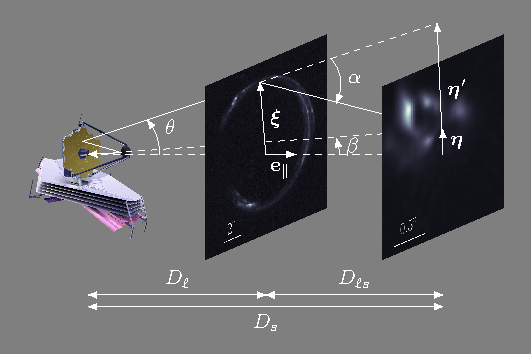
\includegraphics[width=0.7\textwidth]{figures/lensing_cartoon}
        \caption{Schéma d'une lentille gravitationnelle.}
        \label{fig:cartoon}
\end{figure}




